\subsection{功能二 后台人工调度与规则辅助调度}
\owner{许盛凯}
后台调度需要把待出行需求与车辆、司机联系起来。该功能的代表性在于同一操作会改变需求分配、方案确认和车辆运行状态，并要求在生成建议后保留人工确认环节，避免仅生成方案就直接占用运力。

\subsubsection{场景建模}
\begin{table}[H]\centering\small
\caption{后台规则辅助调度用例描述}
\begin{tabularx}{\linewidth}{|P{2cm}|Y|}\hline
用例名称 & UC-A01 生成并确认辅助调度方案\\\hline
参与者 & 已登录后台工作台的管理员\\\hline
前置条件 & 存在待调度需求；车辆和司机信息已录入；规则辅助调度使用空闲且已绑定司机的车辆。\\\hline
触发事件 & 管理员点击界面中的“AI 辅助调度”操作。\\\hline
基本流程 & （1）读取待调度需求；（2）按乘客人数降序排列；（3）依次寻找容量足够的候选车辆及绑定司机；（4）生成待确认建议并展示装载率；（5）管理员核对方案；（6）确认时再次检查关键数据与车辆状态；（7）更新方案、需求、车辆和后台位置记录。\\\hline
异常流程 & 没有候选车辆、没有待调度需求或无法覆盖任何需求时返回提示；方案不存在、已确认或车辆已不空闲时拒绝确认。\\\hline
后置条件 & 成功确认的方案标记为已确认，对应需求为已调度，车辆为运行中，后台新增该车辆位置记录。\\\hline
替代流程 & 管理员手工选择需求、车辆和司机，校验空闲状态、绑定关系与座位容量后生成待确认方案。\\\hline
\end{tabularx}\end{table}
界面沿用“AI 辅助调度”的功能名称，当前实现为可解释的规则匹配。管理员可查看建议并人工确认，现阶段没有调用外部大模型，也没有全局最优调度求解过程。

\subsubsection{类建模}
图\ref{fig:dispatch-class}将需求与调度结果分成两个实体。方案保存需求、车辆和司机的标识以及当次装载率，避免将需求数据直接当作已执行任务。
\begin{figure}[H]\centering
\begin{tikzpicture}[x=1cm,y=1cm]
\node[box,text width=5.9cm] (demand) at (0,0) {\textbf{DispatchDemandModel}\par\rule{5.7cm}{0.3pt}\par\code{id, routeName, passengerCount}\par\code{departureTime, status}};
\node[box,text width=5.9cm] (plan) at (7.3,0) {\textbf{DispatchPlanModel}\par\rule{5.7cm}{0.3pt}\par\code{demandId, vehicleId, driverId}\par\code{loadRate, isConfirmed}\par\code{isAiGenerated}};
\node[box,text width=5.9cm] (v) at (0,-4.0) {\textbf{VehicleModel}\par\rule{5.7cm}{0.3pt}\par\code{id, plateNo, model}\par\code{seatCount, status}};
\node[box,text width=5.9cm] (dr) at (7.3,-4.0) {\textbf{AdminDriverModel}\par\rule{5.7cm}{0.3pt}\par\code{id, name, phone, licenseNo}\par\code{boundVehicleId?}};
\draw (demand.east)--node[font=\scriptsize,above]{1\quad 0..*}(plan.west);
\draw (plan.south west)--node[font=\scriptsize,above,sloped,pos=.25]{0..*}node[font=\scriptsize,above,sloped,pos=.85]{1}(v.north east);
\draw (plan.south)--node[font=\scriptsize,right,pos=.2]{0..*}node[font=\scriptsize,right,pos=.8]{1}(dr.north);
\draw[dashed] (v.east)--node[font=\scriptsize,above]{绑定}(dr.west);
\end{tikzpicture}
\caption{后台调度核心类模型（历史方案可多次引用资源）}\label{fig:dispatch-class}
\end{figure}

\noindent\textbf{类之间的关系。}\code{DispatchDemandModel}保存路线、人数、时间和需求状态；\code{DispatchPlanModel}保存匹配结果、生成方式与确认标记；\code{VehicleModel}描述车辆容量与运行状态；\code{AdminDriverModel.boundVehicleId}描述可选的车辆绑定。\code{AdminController}统一完成查找、校验和状态替换。

\subsubsection{功能建模/行为建模}
图\ref{fig:dispatch-flow}概括建议生成和确认的活动流程。生成阶段使用集合记录本批次已匹配的车辆，防止一辆车在同一批建议中被重复使用；未找到适配车辆的需求保留待调度状态。
\begin{figure}[H]\centering
\begin{tikzpicture}[node distance=0.45cm,font=\small]
\node[state,text width=8cm,inner sep=4pt] (a) {读取空闲且绑定司机的候选车辆};
\node[state,text width=8cm,inner sep=4pt,below=of a] (b) {待调度需求按人数降序排序};
\node[state,text width=8cm,inner sep=4pt,below=of b] (c) {依次匹配容量足够且本批尚未使用的车辆};
\node[state,text width=8cm,inner sep=4pt,below=of c] (d) {生成待确认建议，记录车辆使用情况\par 无法匹配的需求保持待调度};
\node[state,text width=8cm,inner sep=4pt,below=of d] (e) {展示路线、司机、车辆和装载率\par 等待管理员确认};
\node[state,text width=8cm,inner sep=4pt,below=of e] (f) {复核方案、关联数据与车辆空闲状态};
\node[state,text width=8cm,inner sep=4pt,below=of f] (g) {确认方案；需求已调度；车辆运行中\par 建立后台车辆位置记录};
\foreach \s/\t in {a/b,b/c,c/d,d/e,e/f,f/g} \draw[flow] (\s)--(\t);
\node[box,align=center,text width=2.15cm,right=1.0cm of b] (err) {无候选或\par 无待调度需求\par 返回提示};
\draw[flow] (a.east)-| (err.north);
\draw[flow] (b.east)--(err.west);
\node[box,align=center,text width=2.15cm,right=1.0cm of f] (err2) {复核失败\par 拒绝确认\par 提示原因};
\draw[flow] (f.east)--(err2.west);
\end{tikzpicture}
\caption{规则辅助调度与人工确认活动流程}\label{fig:dispatch-flow}
\end{figure}

规则按需求人数降序逐项匹配，选择候选集合中首个容量足够且本批未用的车辆。装载率按“需求人数/车辆座位数”计算。该规则便于解释和演示，但结果会受候选车辆顺序影响，尚未覆盖多车拆分、时间冲突和路线成本等约束。

确认操作与建议生成分开：确认时检查方案是否存在、是否已确认、需求/车辆/司机是否仍存在及车辆是否空闲。成功后一次性替换后台状态中的相关列表。后续接入共享服务端时，还需对需求重复分配、司机冲突和并发确认进行更完整的事务校验。

\subsubsection{代码结构及说明}
\begin{table}[H]\centering\small
\caption{调度功能代码结构与职责}
\begin{tabularx}{\linewidth}{|P{2.1cm}|Y|}\hline
层次 & 文件与职责\\\hline
页面层 & \code{lib/features/admin/presentation/admin_home_page.dart}：待调度需求、人工调度对话框、建议卡片和确认入口。\\\hline
状态层 & \code{lib/features/admin/providers/admin_provider.dart}：车辆司机维护、调度建议生成、方案确认和位置模拟。\\\hline
数据层 & \code{lib/features/admin/data/mock_admin_repository.dart}：提供演示车辆、司机、需求、位置与分析快照。\\\hline
模型层 & \code{lib/core/models/dispatch_model.dart}、\code{vehicle_model.dart}、\code{admin_driver_model.dart}和\code{vehicle_location_model.dart}。\\\hline
\end{tabularx}\end{table}

\noindent\textbf{关键操作。}\code{generateAiDispatchPlans}生成规则建议；\code{createManualDispatchPlan}处理人工选择；\code{confirmDispatchPlan}执行确认。规则匹配的核心片段如下：
\begin{source}
final sortedDemands = [...state.pendingDispatchDemands]
  ..sort((a, b) => b.passengerCount.compareTo(a.passengerCount));
final usedVehicleIds = <String>{};
for (final demand in sortedDemands) {
  final pair = candidates.where((item) {
    return !usedVehicleIds.contains(item.vehicle.id) &&
        item.vehicle.seatCount >= demand.passengerCount;
  }).firstOrNull;
  if (pair == null) continue;
  usedVehicleIds.add(pair.vehicle.id);
  // Build one pending plan with demand, vehicle and driver.
}
\end{source}
\noindent 片段中的候选集合由\code{_availableVehicleDriverPairs}构造。方法只纳入空闲且已有绑定司机的车辆；人工调度则允许在通过绑定检查的情况下选择未绑定司机，确认时再建立绑定。

\noindent\textbf{阶段验证。}已有测试覆盖人工方案、建议生成、确认，以及无可用车辆和座位不足等失败分支。当前确认只更新后台模块的内存数据，尚不会自动向乘客端创建车次或向司机端推送任务。下一阶段将统一这三种业务对象的标识与接口，并补充重复需求、车辆状态变化和司机占用冲突的测试。

\clearpage
\subsubsection{界面截图}
\begin{figure}[H]\centering
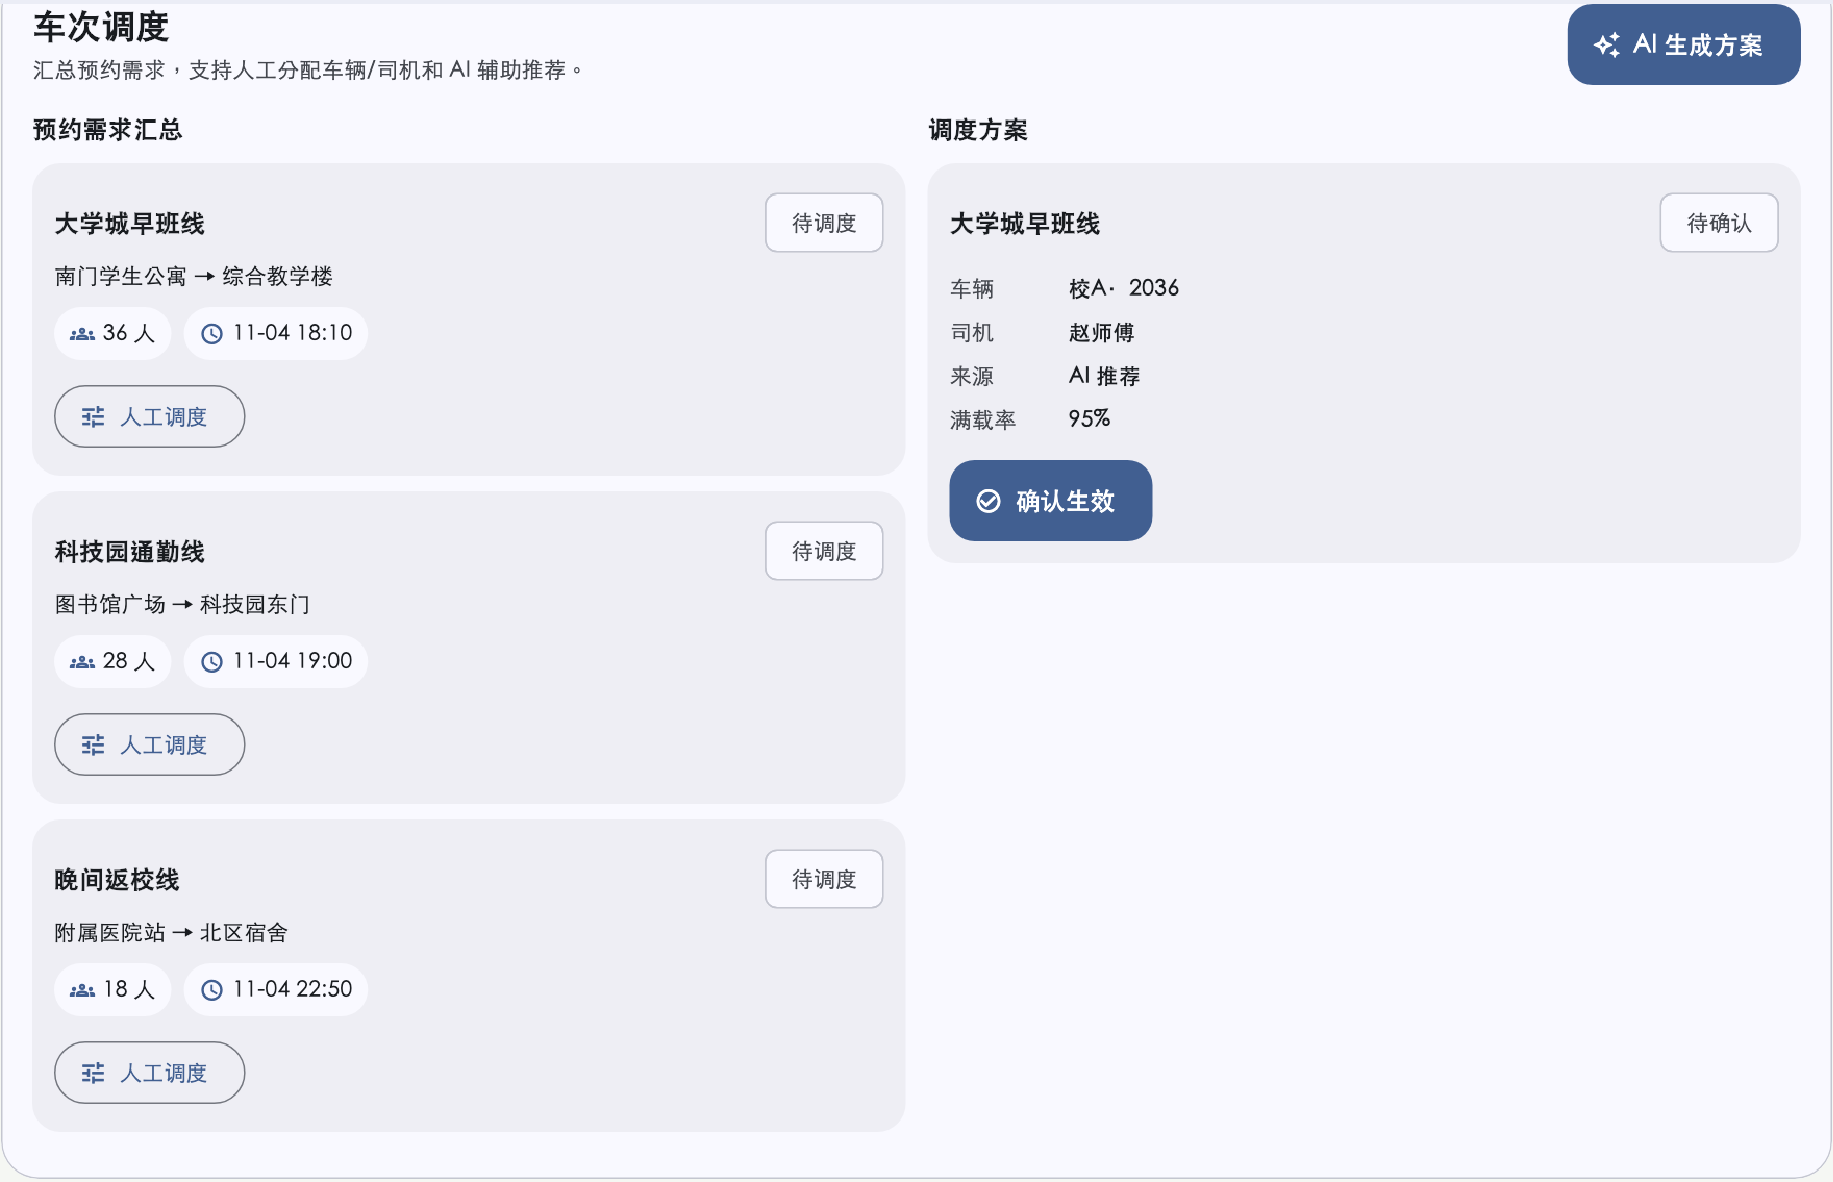
\includegraphics[width=\linewidth,height=0.64\textheight,keepaspectratio]{figures/dispatch.pdf}
\caption{后台生成调度建议并等待人工确认的运行界面}\label{fig:dispatch-screen}
\end{figure}

调度界面将需求信息与建议结果分区展示。管理员可以核对路线、发车时间、乘客人数、车辆、司机与装载率，再点击确认；人工调度则通过对话框逐项选择资源，使规则建议与人工处理共用同一确认流程。

现阶段后台已经形成“维护运力—生成方案—人工确认—查看状态”的本地操作流程。后续重点是完善确认前的约束复核，并将确认结果映射为统一车次和司机任务，逐步完成真实数据条件下的跨端联调。
